\section{Nigredo, Albedo and Rubedo}
\label{sec:NigredoAlbedoandRubedo}

Imagine the life of a contemporary version of “Snow White”. The Evil Queen still wants to kill her stepdaughter. But she has learned from her previous mistakes and got the seven dwarves to abandon their mine. Instead, they are roaming the lands of World of Warcraft, because the Queen made them regard their hard labour as an unnecessary relict from some dark, uncivilised past. For reasons of animal welfare, the hunter was banned from hunting and moved away. So what about the Prince? He is nowhere to be found. Rumour has it that he probably never existed in the first place and had only been designed as a distraction to prevent young girls from becoming astrophysicists and CEOs. By removing every male character from the fairy tale, will the Evil Queen finally achieve the death of Snow White?

\paragraph{The Killing of Snow White}
Nobel Laureate Elfriede Jelinek makes short work of Snow White in her drama \emph{Death and the Maiden I}: her hunter shoots Snow White dead. Needless to say, this act of violence is celebrated as a feminist victory over the so-called patriarchal stereotype of beauty and the feminine wish to please. Snow White is dead and women are no longer perceived as beautiful “objects”. If this assertion were to be correct, it would mean that the only force responsible for the “eternal enslavement” of woman is woman herself. So doing away with her is the way out then?

\begin{wrapfigure}{rt}{.3\textwidth}
\centering
 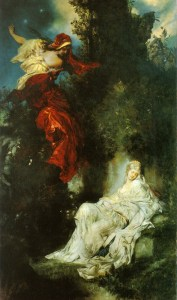
\includegraphics[scale=.6]{a20210127NigredoAlbedoandRubedo-img001.jpg} 
\end{wrapfigure}

In her collection of plays called \emph{Princess dramas}, Jelinek alleges that woman is excluded from truth, because she is incapable of knowing herself as a “subject”. She further states: “[My] texts are partly very philosophic, they make fun of the philosophy of Heidegger, because the areas where woman has been excluded the most have always been thinking and music.” In other words: killing Snow White wasn't enough for Jelinek, she also wishes to exclude woman from Western heritage by negating the very point of music and thinking — i.e., the inclusion of woman into the hearts and minds of men.

In defence of Jelinek one could argue that she might not have had much of a choice other than to kill her inner Snow White in order to survive the harassment by her own mother. If faced with the envy of an Evil Queen and no male rescuers at hand, what is Snow White supposed to do if she wants to stay alive? So before condemning Jelinek for her brutality one has to acknowledge that the death of Snow White could have been her last resort. If the feature that constitutes Snow White's existence is a crime, she simply cannot exist. Matriarchy means the extinction of Snow White as well as the Prince — that is to say: the extinction of love.

\paragraph{Transformation}
\begin{quotex}
But I have no time for such things; and the reason, my friend, is this. I am still unable, as the Delphic inscription orders, to know myself; and it really seems to be ridiculous to look into other things before I have understood that. \flright{\textsc{Plato}, \emph{Phaedrus}}

\end{quotex}
The list of psychological analyses of Snow White is long, rumours about a Rosicrucian origin of the symbolism are widespread — I am not going to recount them here. I would rather like to dismiss the superficial notion that the story is merely about a mother-daughter conflict which will be resolved once Snow White grows up, ceases to be an object of pleasure and finally gets hold of the keys to her own “subjectivity“. The impossibility of being Snow White arises from the Evil Queen's desire for subjectivity. She cannot tolerate beauty that has no intention of its own. Snow White does not suffer from a lack of subjectivity. Under the tyranny of the Evil Queen she is nothing but subjectivity. Without men to marvel at her beauty, to turn her into an object, to save her from death and no dwarves to take care of, she will never be able to “transform” — and fulfil the destiny of the fairy tale.

I am really no expert on alchemy, but in order to achieve “transformation“ you need to do something to a substance. If Snow White is supposed to transform from “nigredo” to “albedo “ to “rubedo“, she needs an impulse from the outside. There is no way for her to develop, if she cannot experience herself as an object. However, it is certainly not the Evil Queen who will bring that change about: her poisoned “gifts” are only meant to encourage vanity and tie Snow White ever closer to her matriarchic rule of total subjectivity.

What possibilities does Snow White have without the hunter, the dwarves and the Prince? How is she supposed to relate to the world if nobody relates to her? There is simply no Snow White left to write a fairy tale about. Without the “transformation” of the subject into an object — dialectic — there would be no “fourth kind of madness” in \emph{Phaedrus}, no pity with Francesca da Rimini in Dante's \emph{Commedia}, no path to any kind of knowledge beyond personal emotions and opinions.

\paragraph{Marcela}
Maybe the “post-structuralist” writer Jelinek sincerely believes subjects have a story of their own. But wasn't it Jelinek's compatriot Wittgenstein who showed that the “thinking, imagining subject” does not exist? That the “I” as a subject remains unattainable for thought because it constitutes “a border of the world”? By killing Snow White Jelinek excluded herself — and as a sophist who is trying to justify her action by claiming the status of a victim, she remains the Evil Queen's most submissive slave.

Now that Snow White has accepted the fact that there will be no hunter, no dwarves and certainly no Prince, she can either become like her tormented and jealous (step)mother or a “sexually emancipated” (Jelinek's self-description), mentally mutilated writer who tries to avoid death by killing herself. So far so good. Maybe there is a third option. Instead of getting bruised by struggling against Wittgenstein's border she could ask Marcela for asylum and accept her own existence without being either ashamed of or sorry for it. Dialectic and devotion can be powerful tools to reduce subjectivity. If she tries really hard, Snow White might manage to transform from “nigredo” to “albedo”. “Rubedo” however will remain out of reach until the Prince finally hears what heaven wills, realises what fate ordains and does his job.

I suppose some would say “rubedo” is dispensable. Those are the ones that tell you the Prince is merely a fantasy and Snow White needs to be killed in order for women to become “subjects”. If “red” were dispensable, Phaedrus would remain without Socrates' second speech and we would know nothing of the “fourth kind of madness”. Some say Marcela represents that fourth kind of madness. Really? Others frame her as the first feminist. Think again: Marcela is the absolute object, completely void of subjectivity and will — thus the negation of the Evil Queen. What the Evil Queen, and Jelinek, fail to grasp, Marcela articulates unmistakably:

\begin{quotex}
until now Heaven has not ordained that I love. And to think that I shall love of my own accord [amar por elección] is to think the impossible. \flright{\textsc{Cervantes}, \emph{Don Quixote}}

\end{quotex}
Love is not a choice. Either you love or you don't, but it is not a decision. You can decide to pursue a relationship with someone. It is a choice to sleep with somebody. You can choose to get married. But to love is not a choice. The choice a woman has to make though is to let go of herself — let go of “subjectivity”. Otherwise she will not recognise love even if a man is on his knees begging for her love. So yes: Snow White actually has to die, not as a victim of the Queen but as a sacrifice to the Prince.

To a woman the love of a man is incomprehensible. She sees it, she hears it, she might enjoy it, be overwhelmed by it and eventually fall in love, but she does not comprehend it. So Marcela is cruel? Is it cruel not to be able to love “of your own accord”? To be unable to feel love unless a man makes you feel it? Why else would music exist? Poetry and art? Are they dispensable? Objects are thought of, written and sung about. Unlike subjects, they are never excluded.


\hfill

The meaning of the alchemical stages are:

\begin{itemize}
\item \textbf{Nigredo}: spiritual death 
\item \textbf{Albedo}: purification 
\item \textbf{Rubedo}: the attainment of a coherent sense of self 
\end{itemize}

\flrightit{Posted on 2021-01-27 by Sibylle }
